\section{Comparison in regard to the Existence of Similar Triples in the Trainings Data}
\label{appendix:similar_triples}

\subsection{Binary}

\begin{figure}[H]
\centering
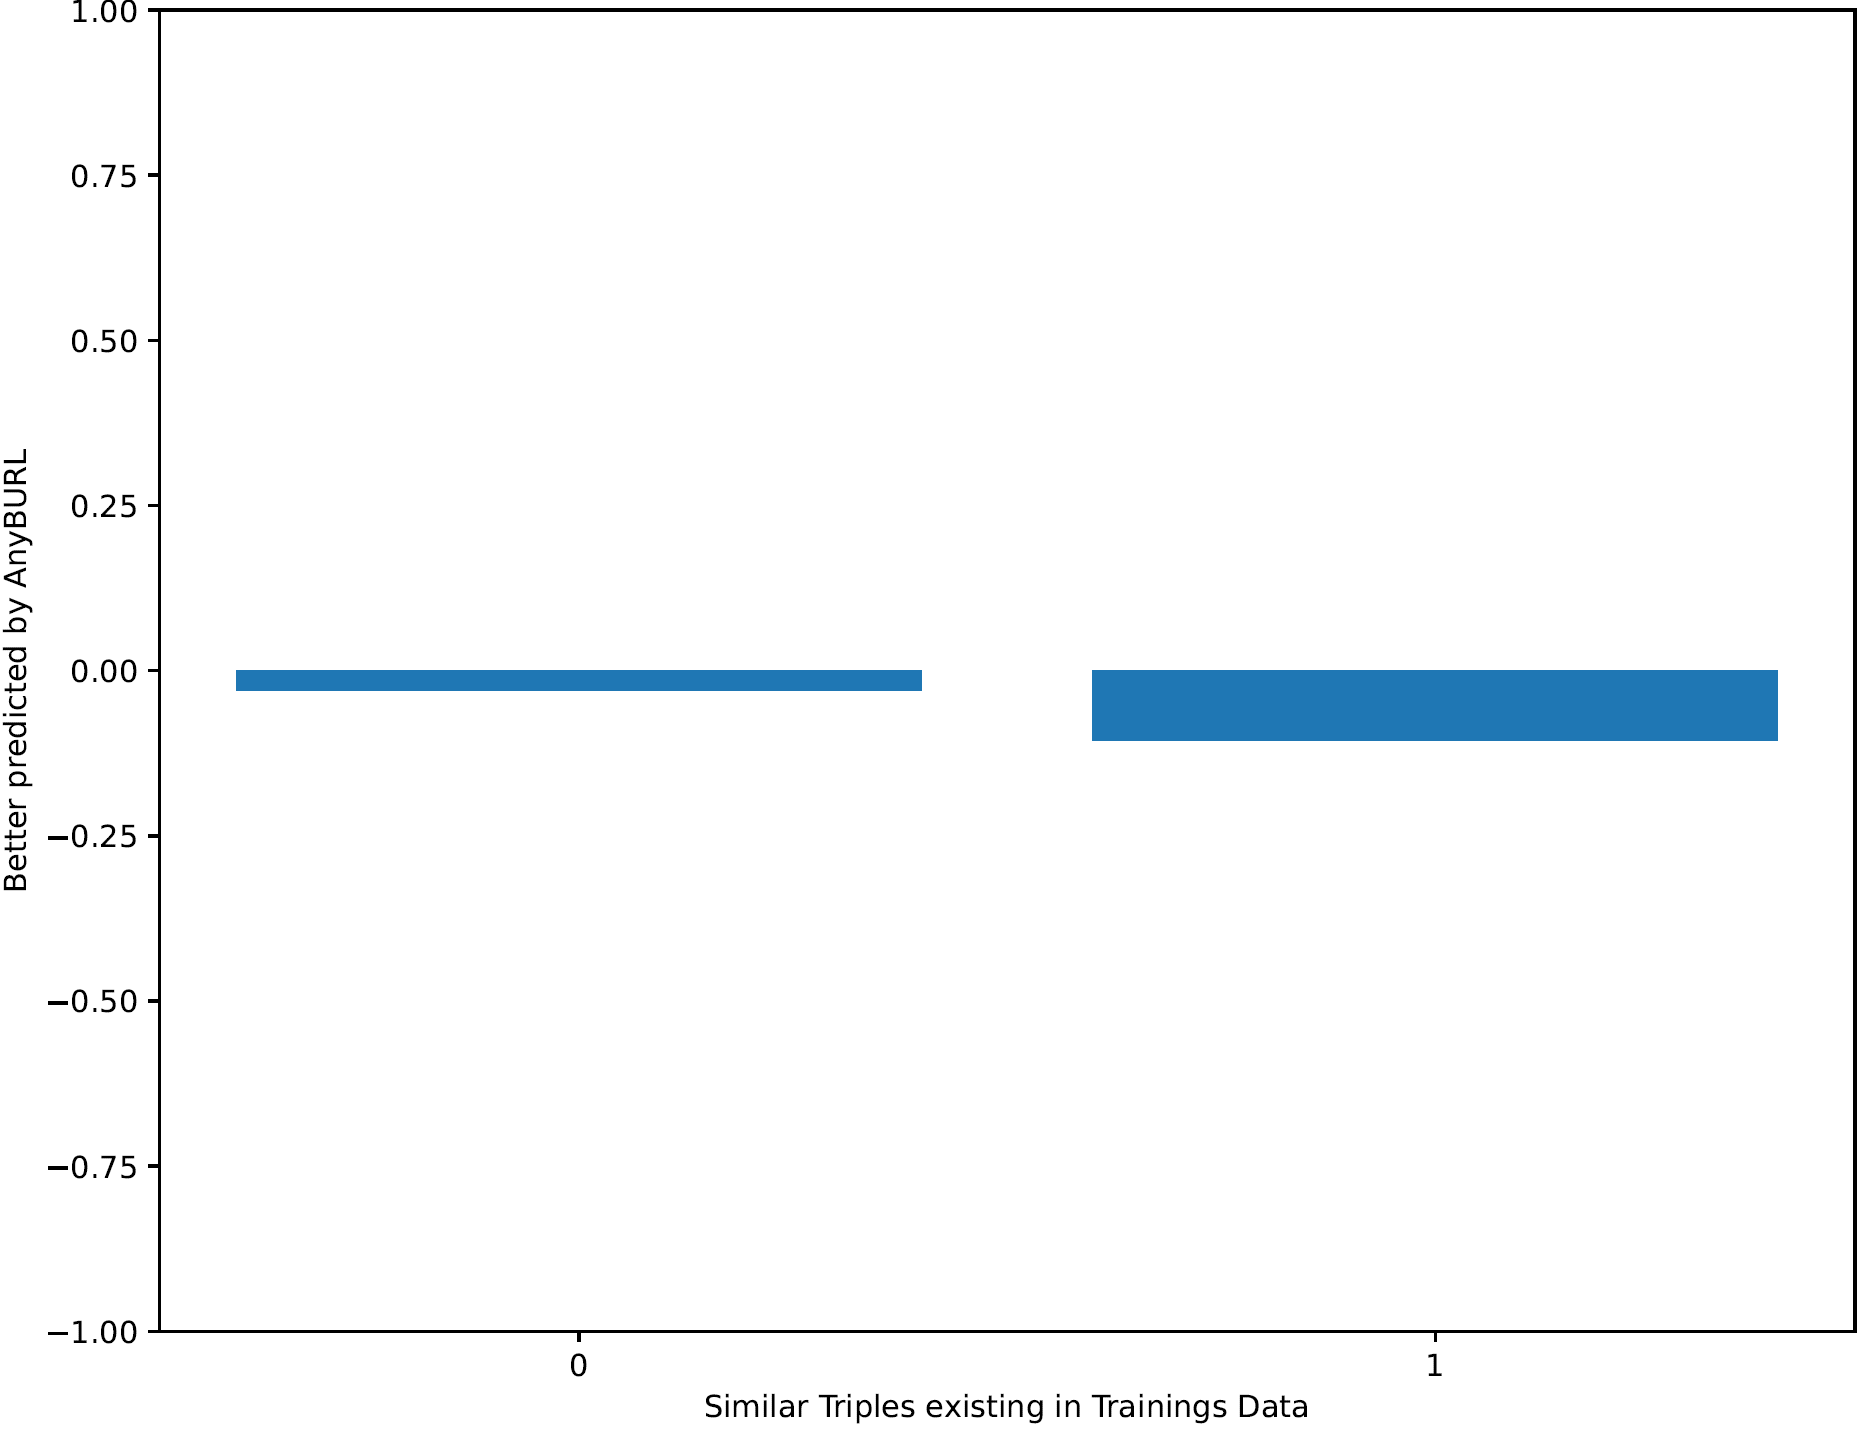
\includegraphics[width=0.7\textwidth]{images/similar_triples_binary_anyburl_conve_codex.PNG}
\caption{Comparison of AnyBURL and ConvE on FB15k-237 in regard to the existence of similar triples in the trainings data}
\label{fig:similar_triples_binary_anyburl_conve_fb15k}
\end{figure}

\begin{figure}[H]
\centering
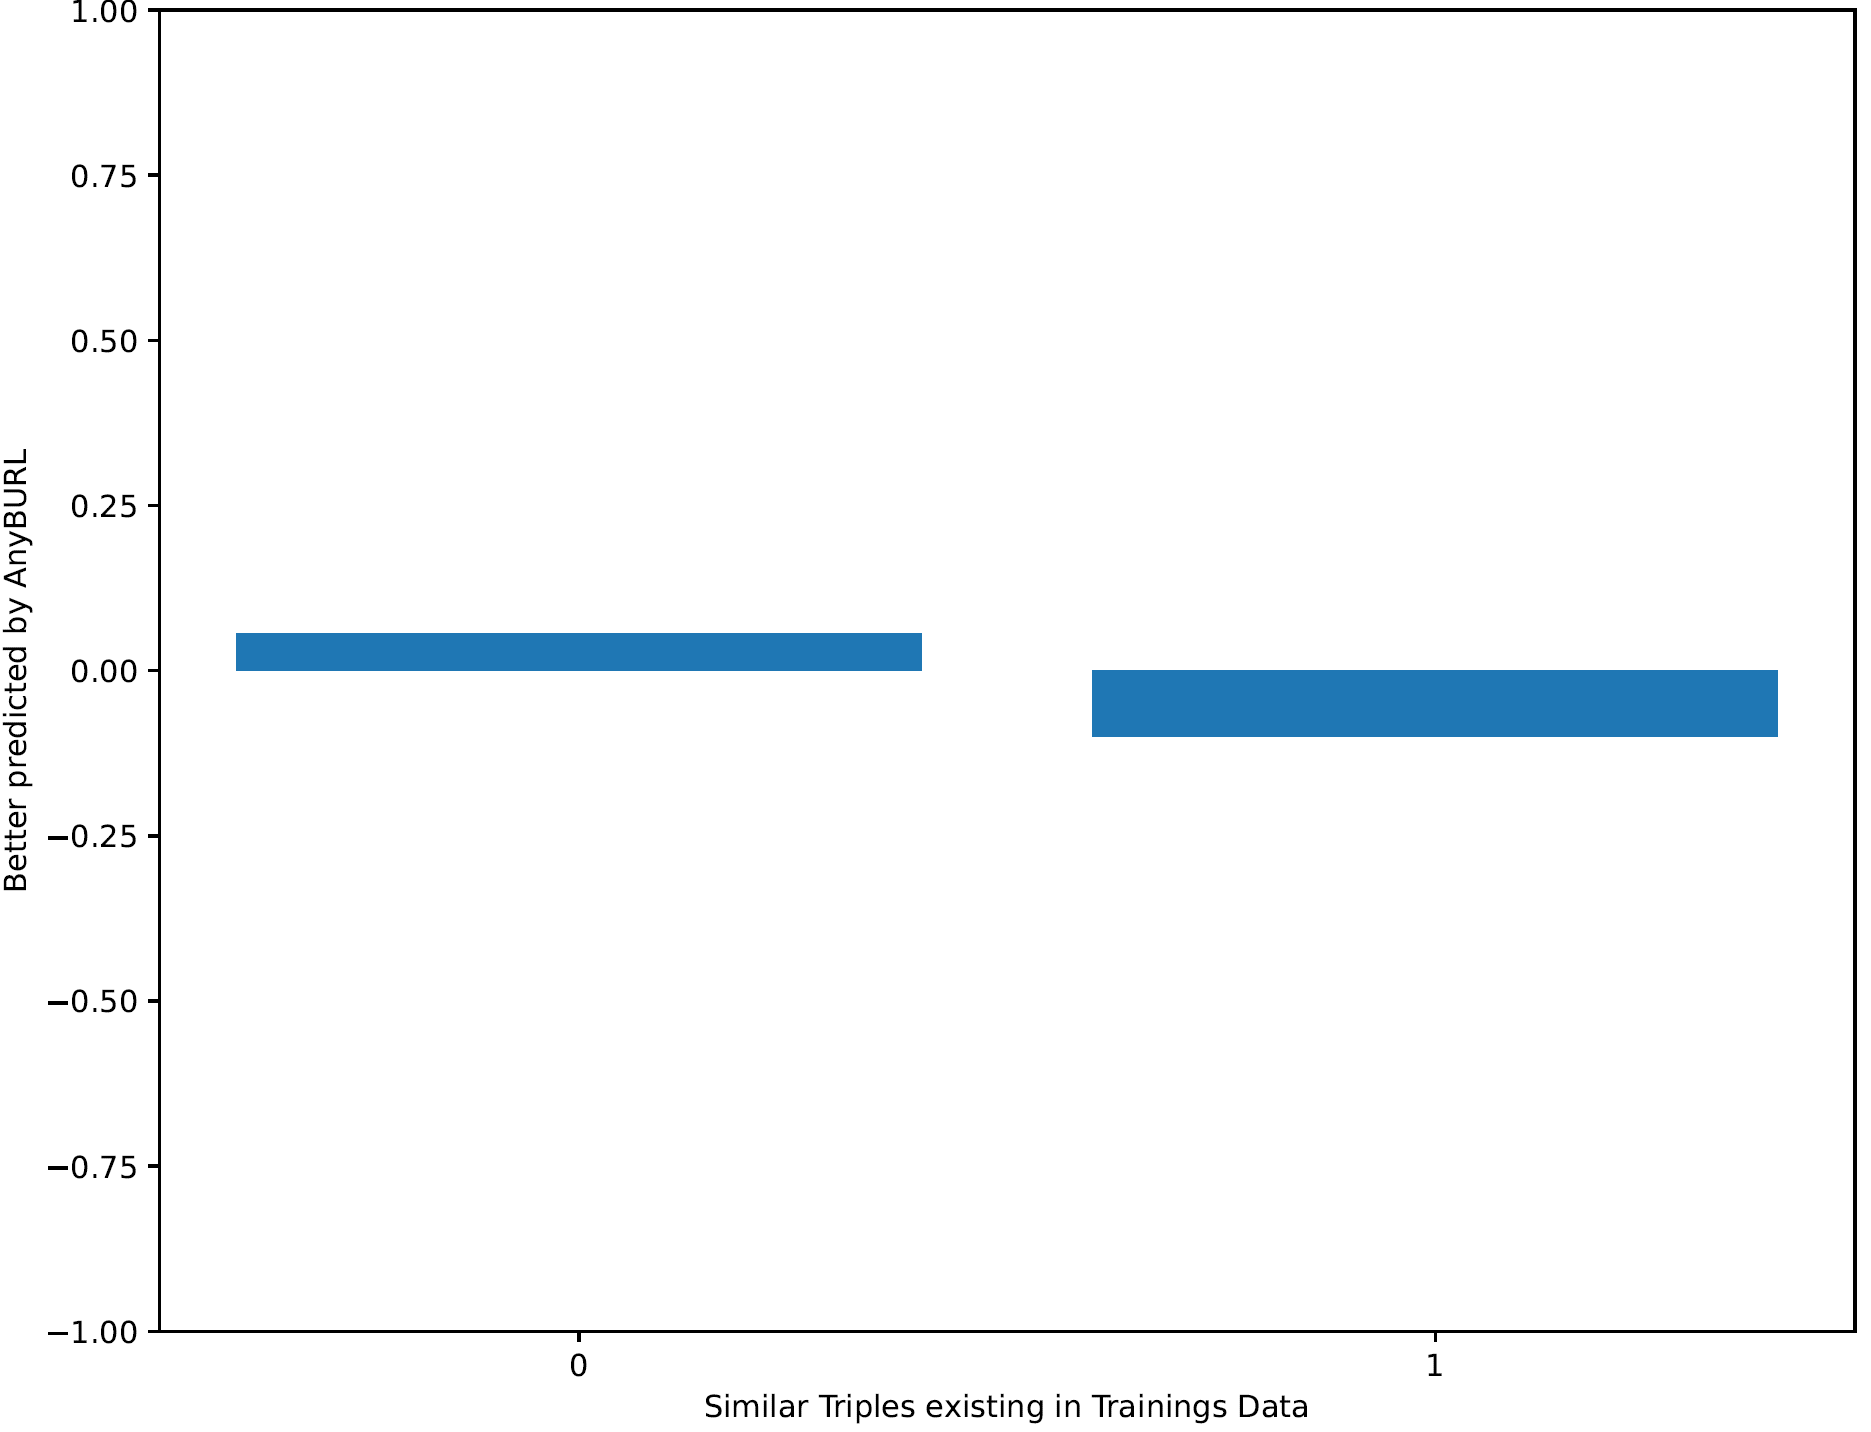
\includegraphics[width=0.7\textwidth]{images/similar_triples_binary_anyburl_rescal_codex.PNG}
\caption{Comparison of AnyBURL and RESCAL on FB15k-237 in regard to the existence of similar triples in the trainings data}
\label{fig:similar_triples_binary_anyburl_rescal_fb15k}
\end{figure}

\begin{figure}[H]
\centering
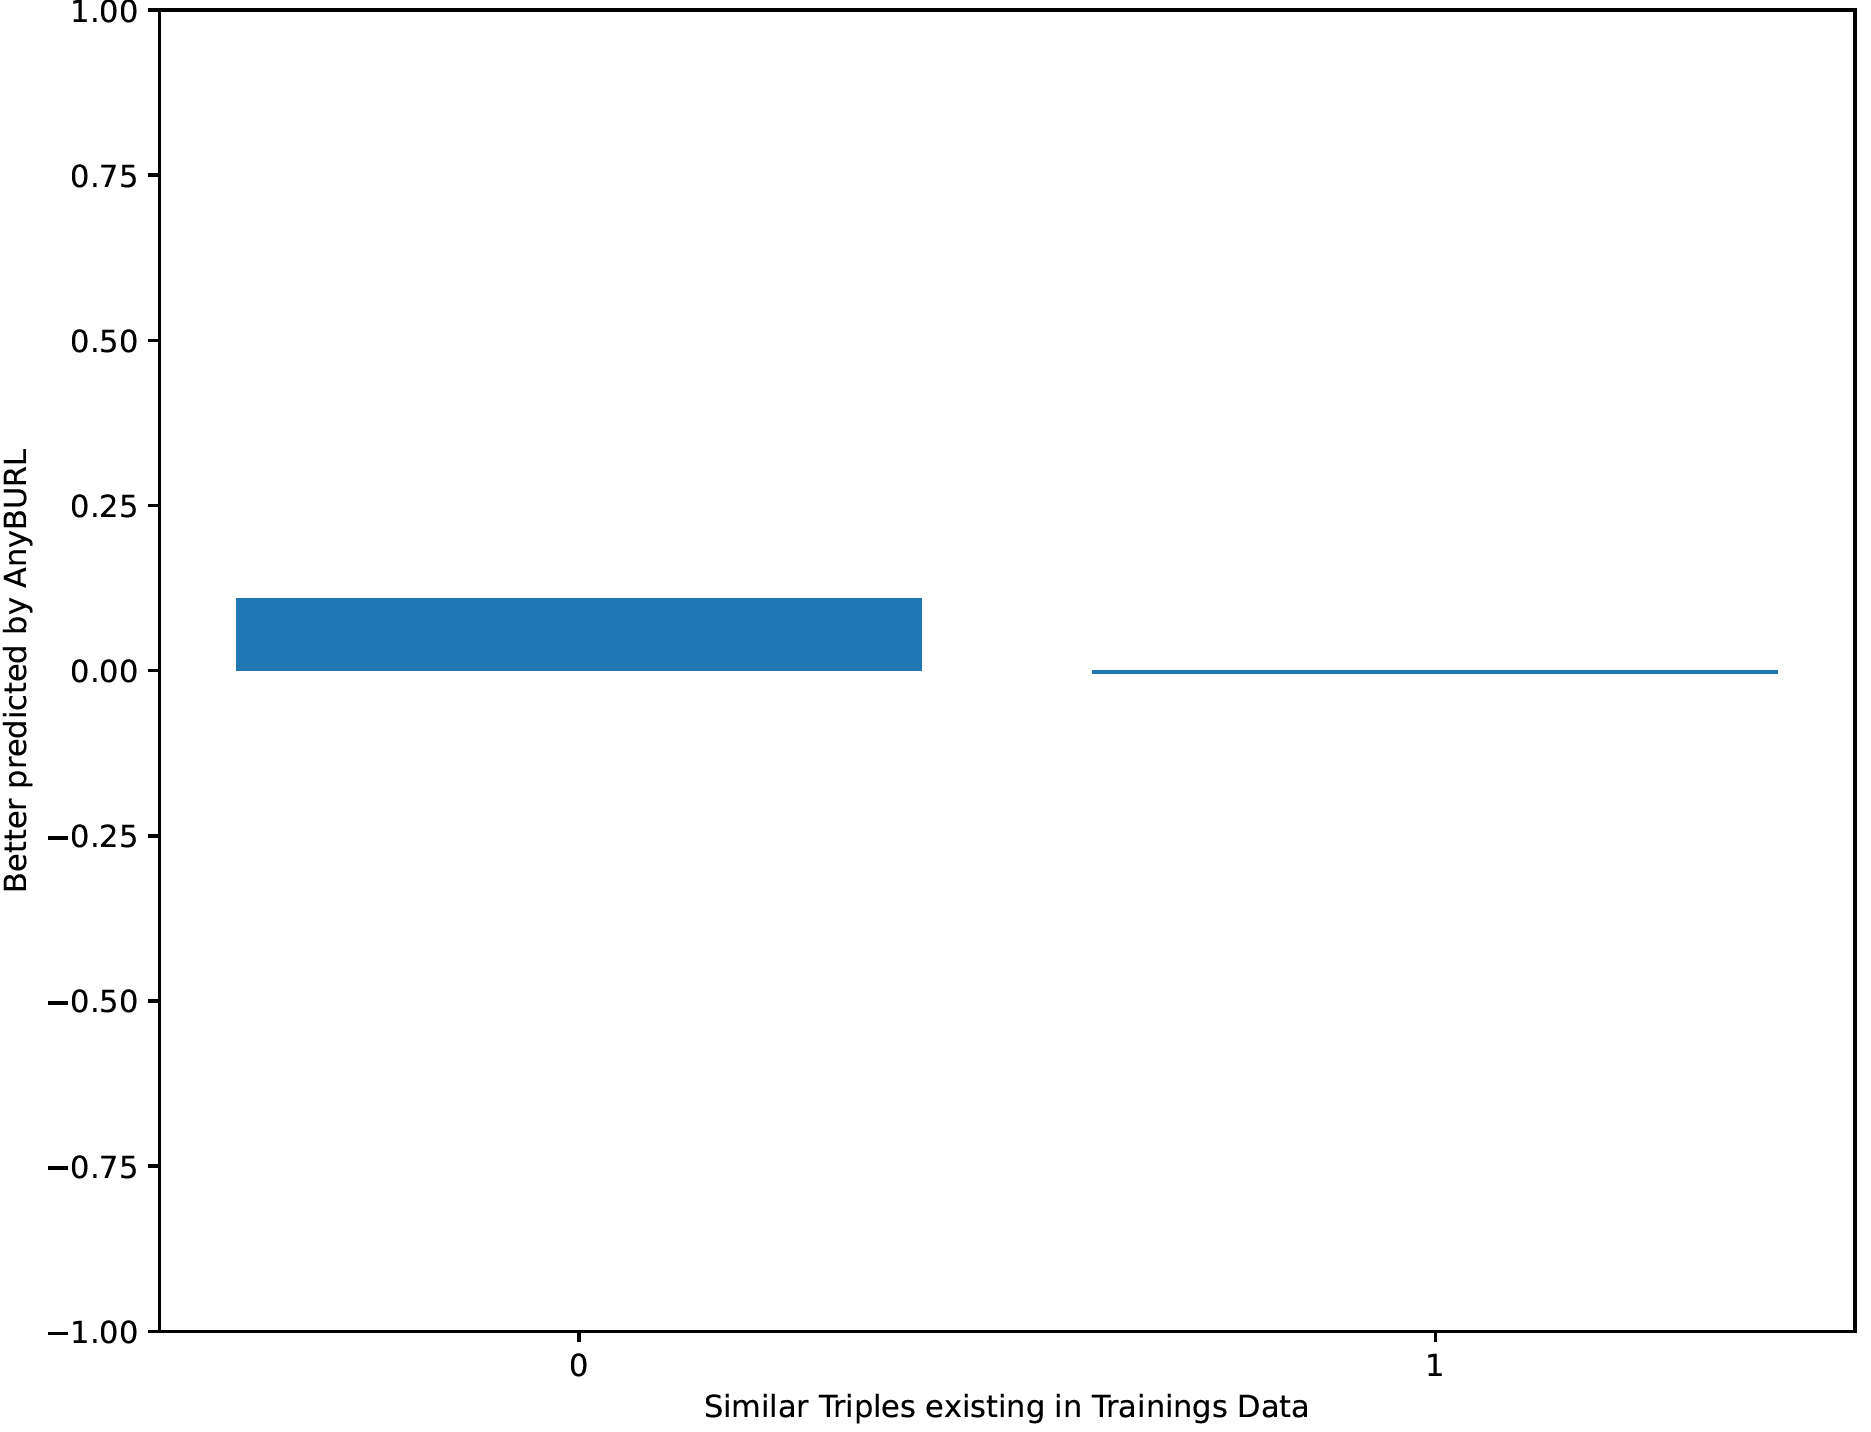
\includegraphics[width=0.7\textwidth]{images/similar_triples_binary_anyburl_complex_yago.PNG}
\caption{Comparison of AnyBURL and ComplEx on YAGO3-10 in regard to the existence of similar triples in the trainings data}
\label{fig:similar_triples_binary_anyburl_complex_yago}
\end{figure}

\subsection{Stepwise}

\begin{figure}[H]
\centering
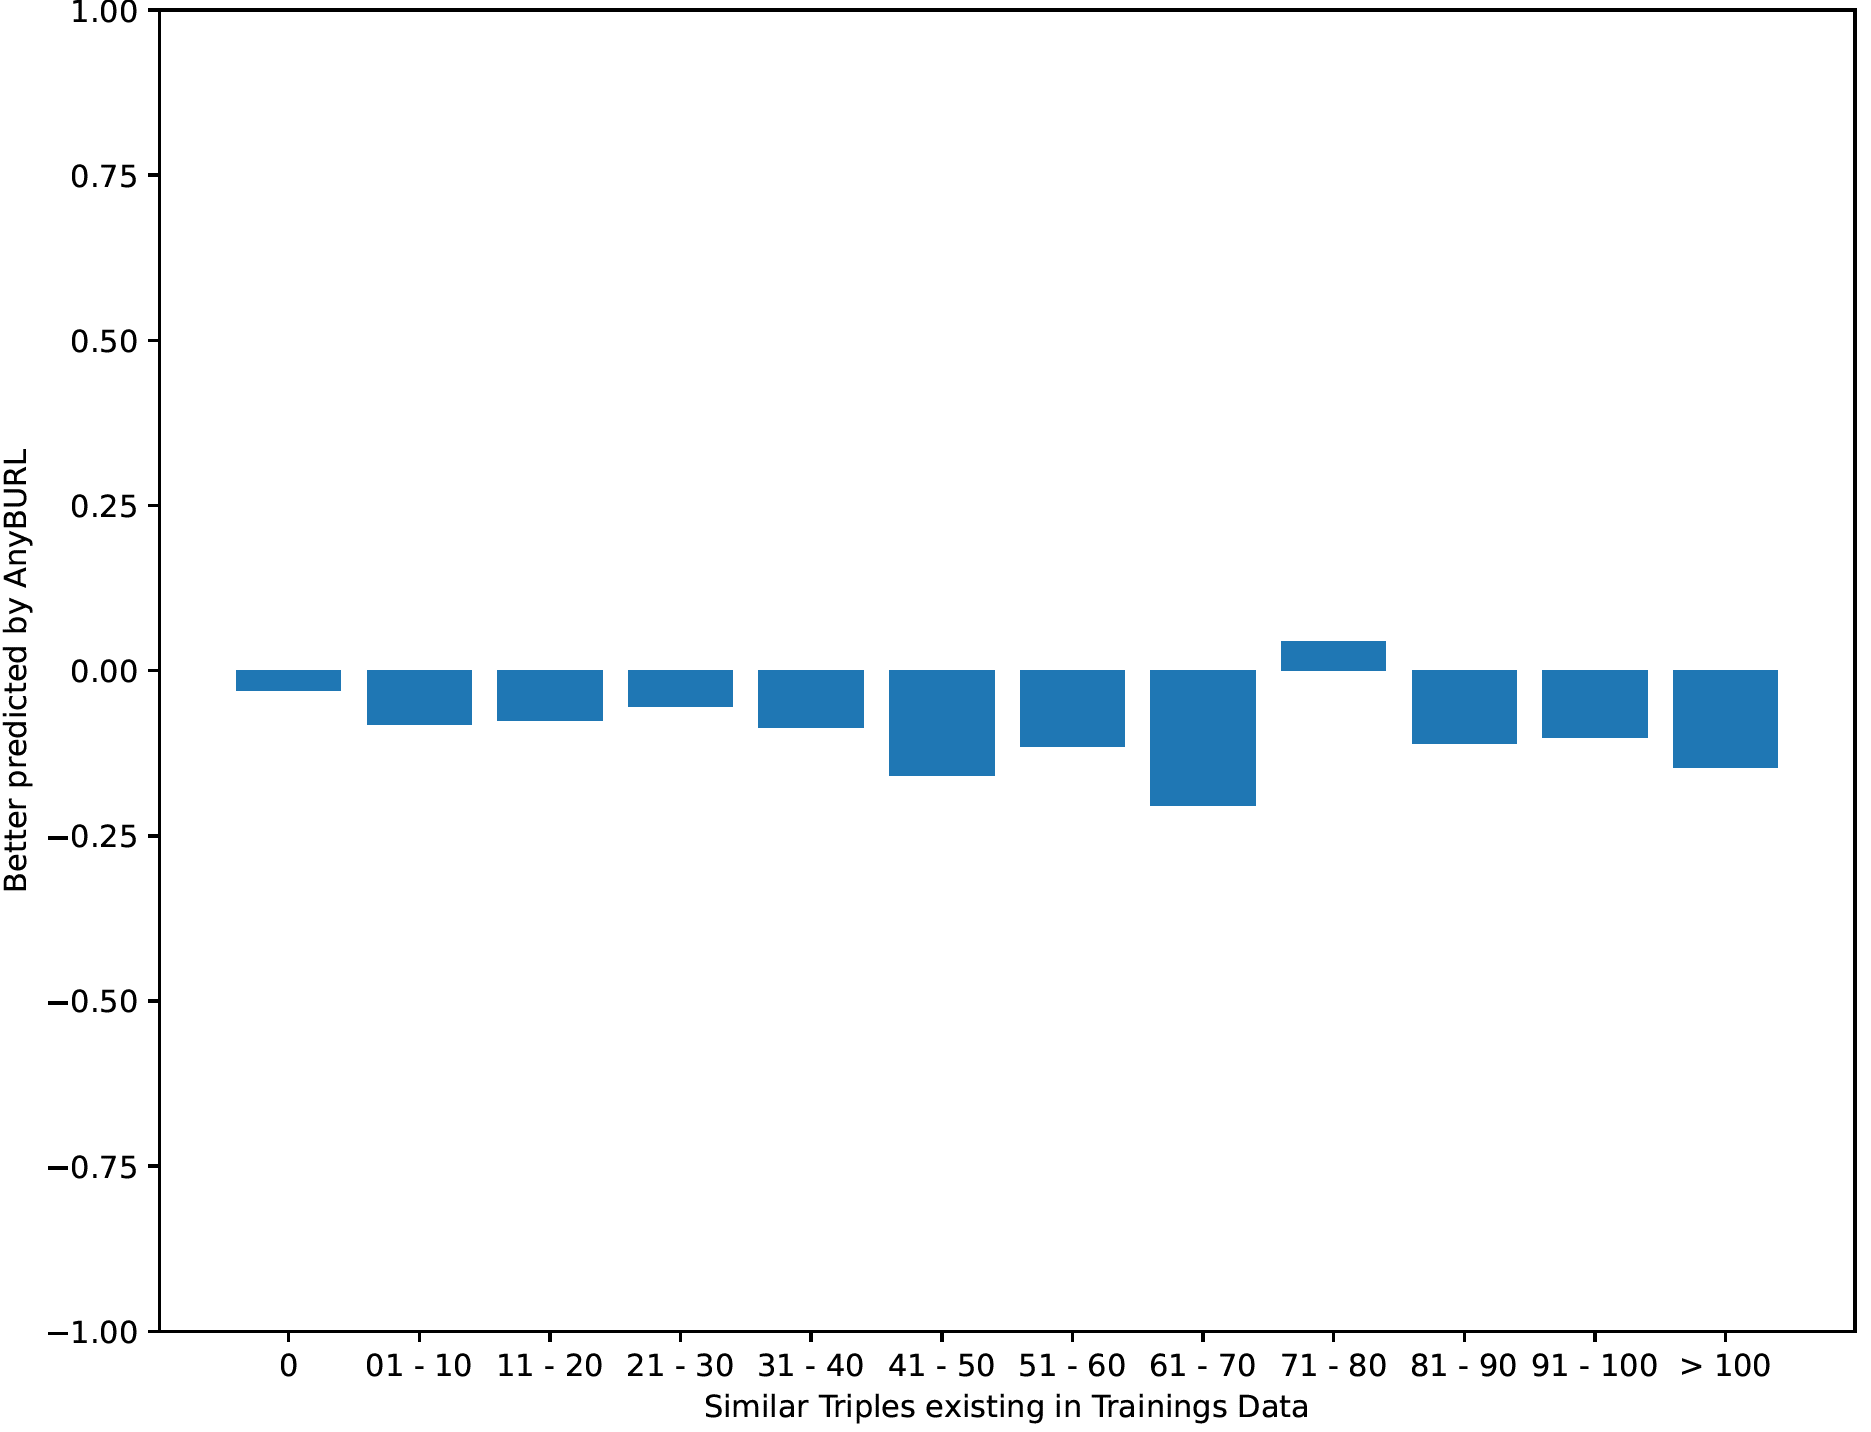
\includegraphics[width=0.7\textwidth]{images/similar_triples_steps_anyburl_conve_codex.PNG}
\caption{Comparison of AnyBURL and ConvE on CodEx-M in regard to the amount of similar triples in the trainings data}
\label{fig:similar_triples_steps_anyburl_conve_codex}
\end{figure}

\begin{figure}[H]
\centering
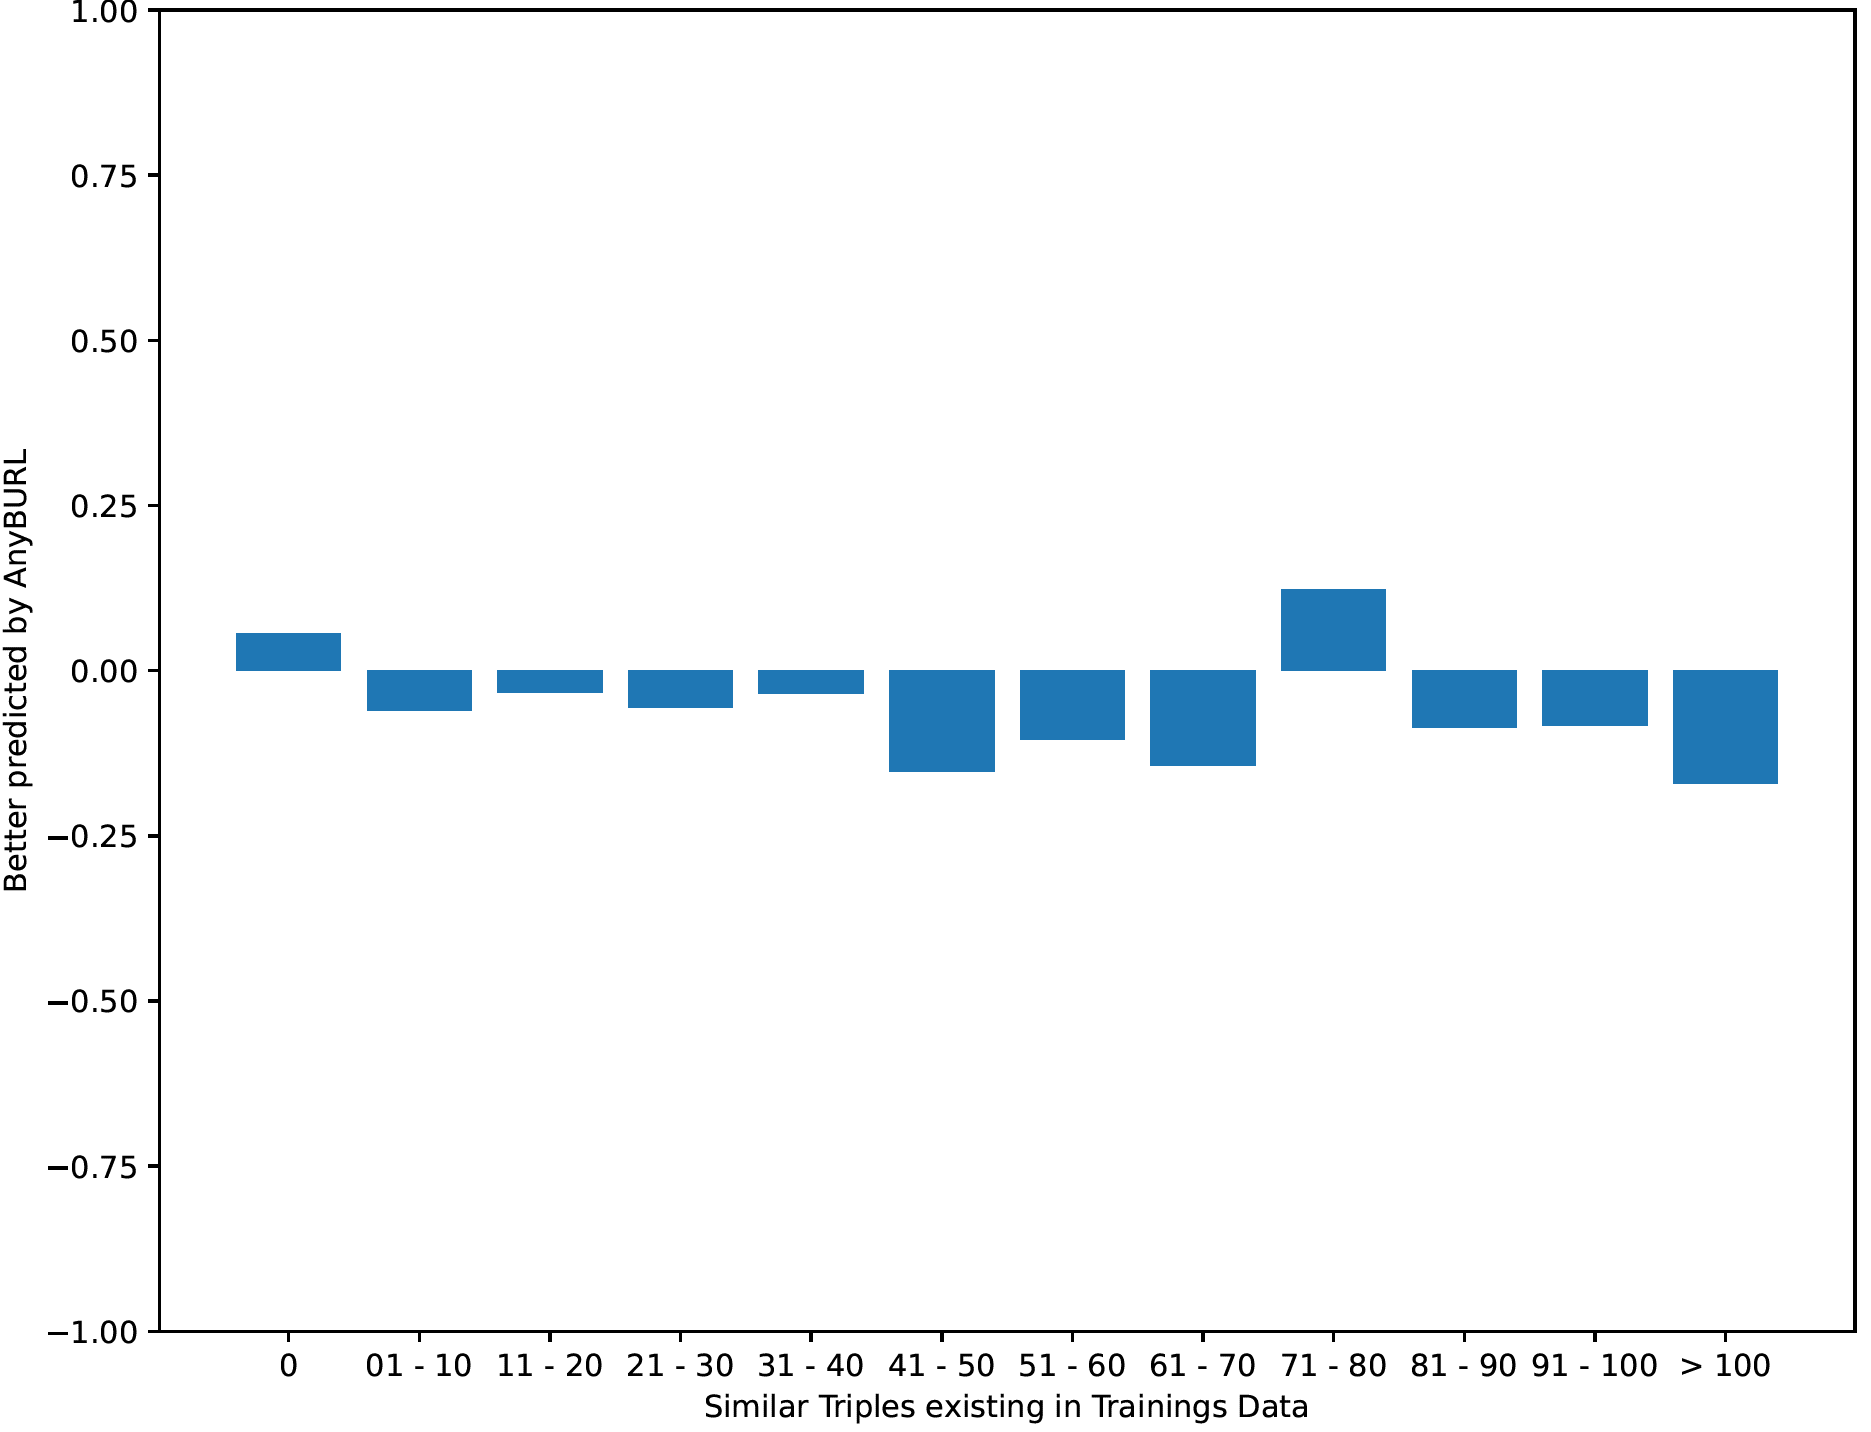
\includegraphics[width=0.7\textwidth]{images/similar_triples_steps_anyburl_rescal_codex.PNG}
\caption{Comparison of AnyBURL and RESCAL on CodEx-M in regard to the amount of similar triples in the trainings data}
\label{fig:similar_triples_steps_anyburl_rescal_codex}
\end{figure}

\begin{figure}[H]
\centering
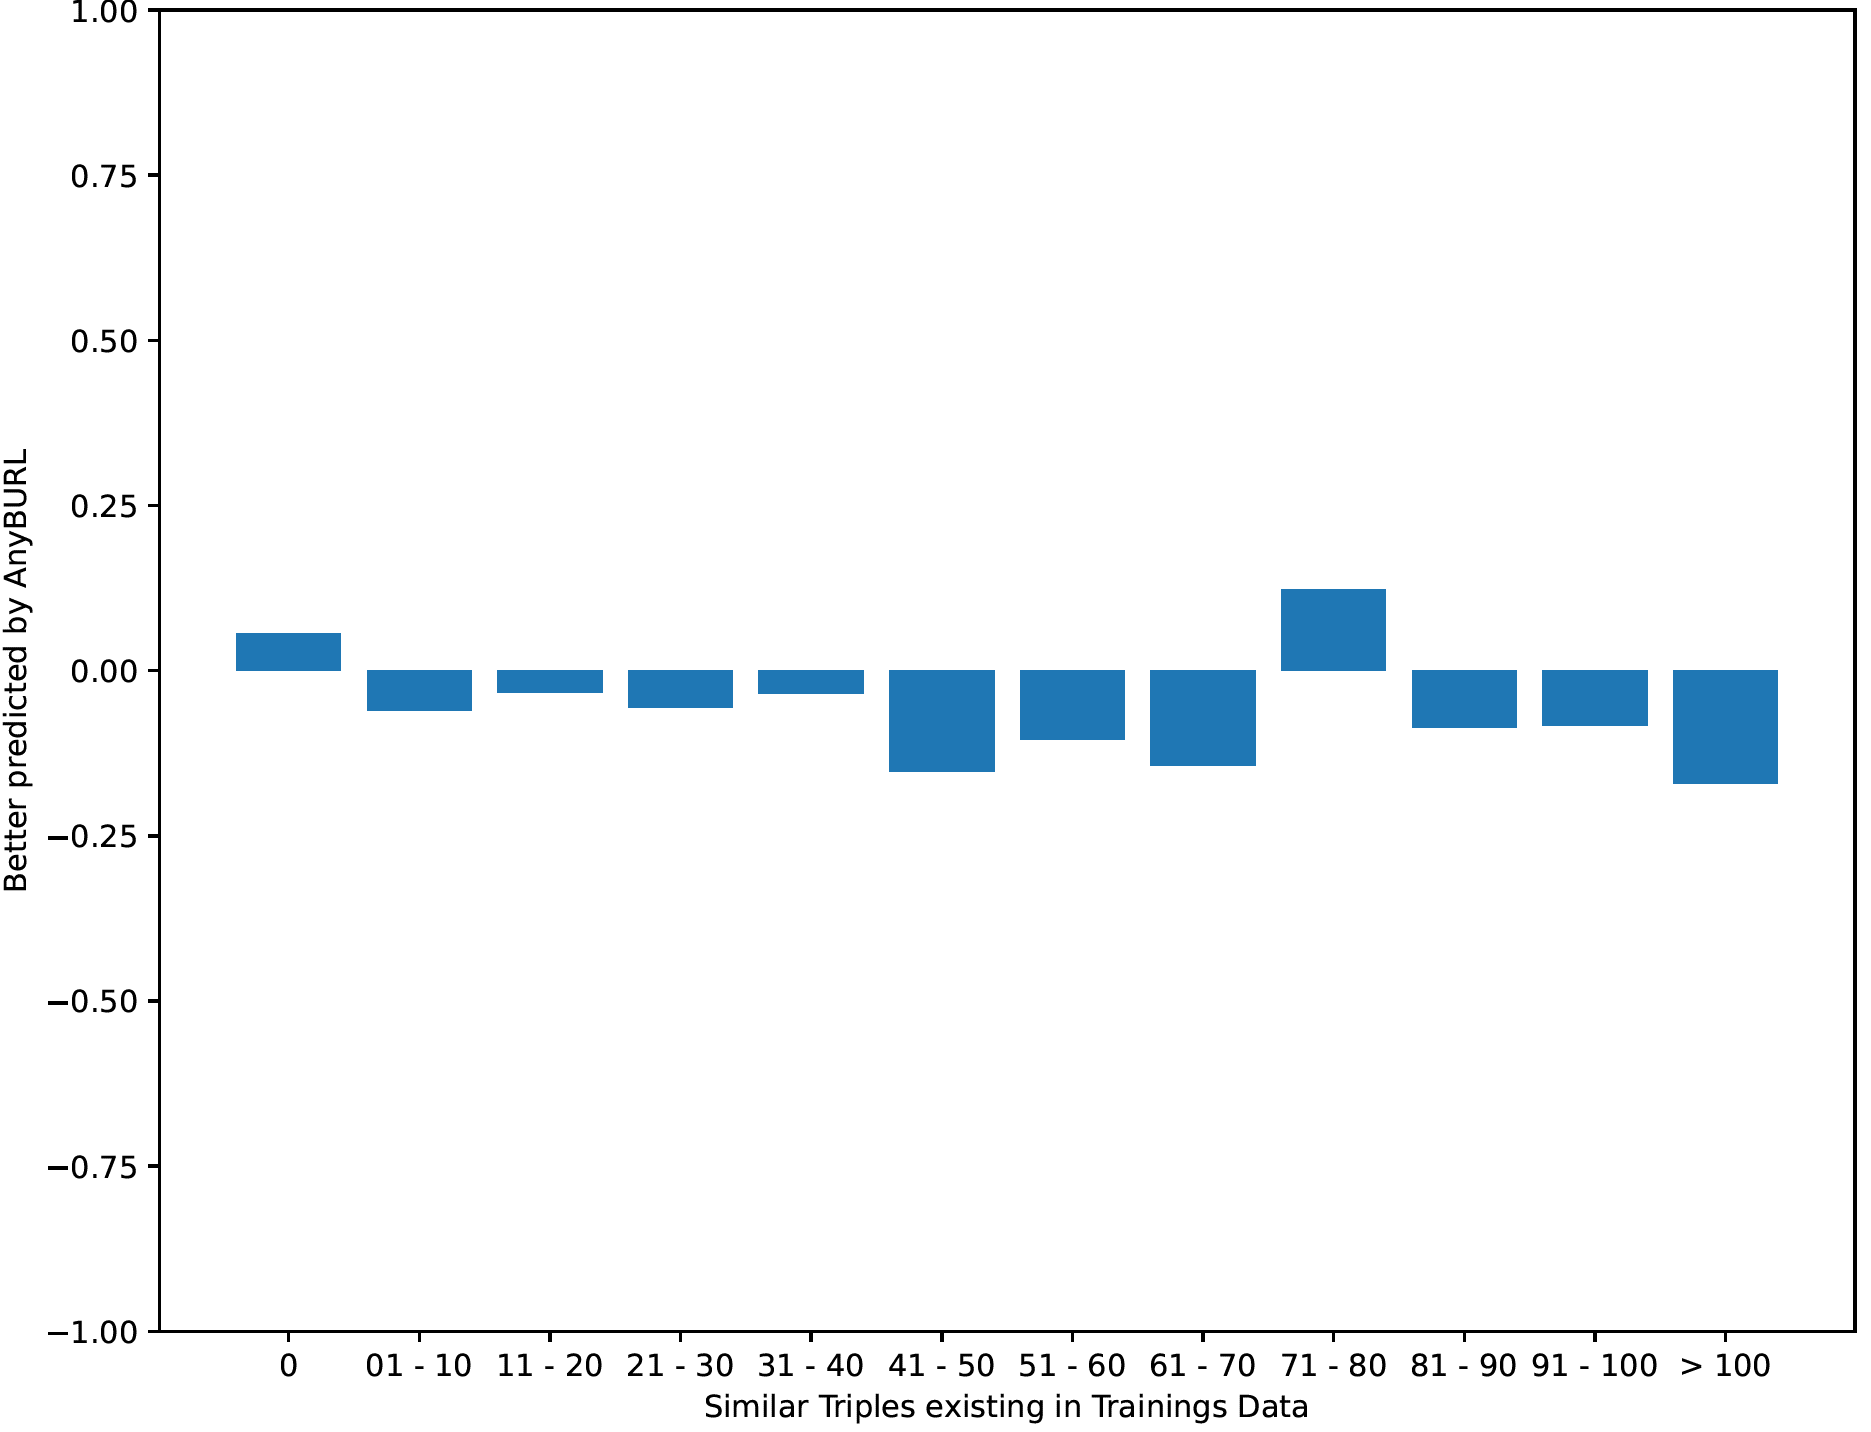
\includegraphics[width=0.7\textwidth]{images/similar_triples_steps_anyburl_complex_fb15k.PNG}
\caption{Comparison of AnyBURL and ComplEx on FB15k-237 in regard to the amount of similar triples in the trainings data}
\label{fig:similar_triples_steps_anyburl_complex_fb15k}
\end{figure}

\begin{figure}[H]
\centering
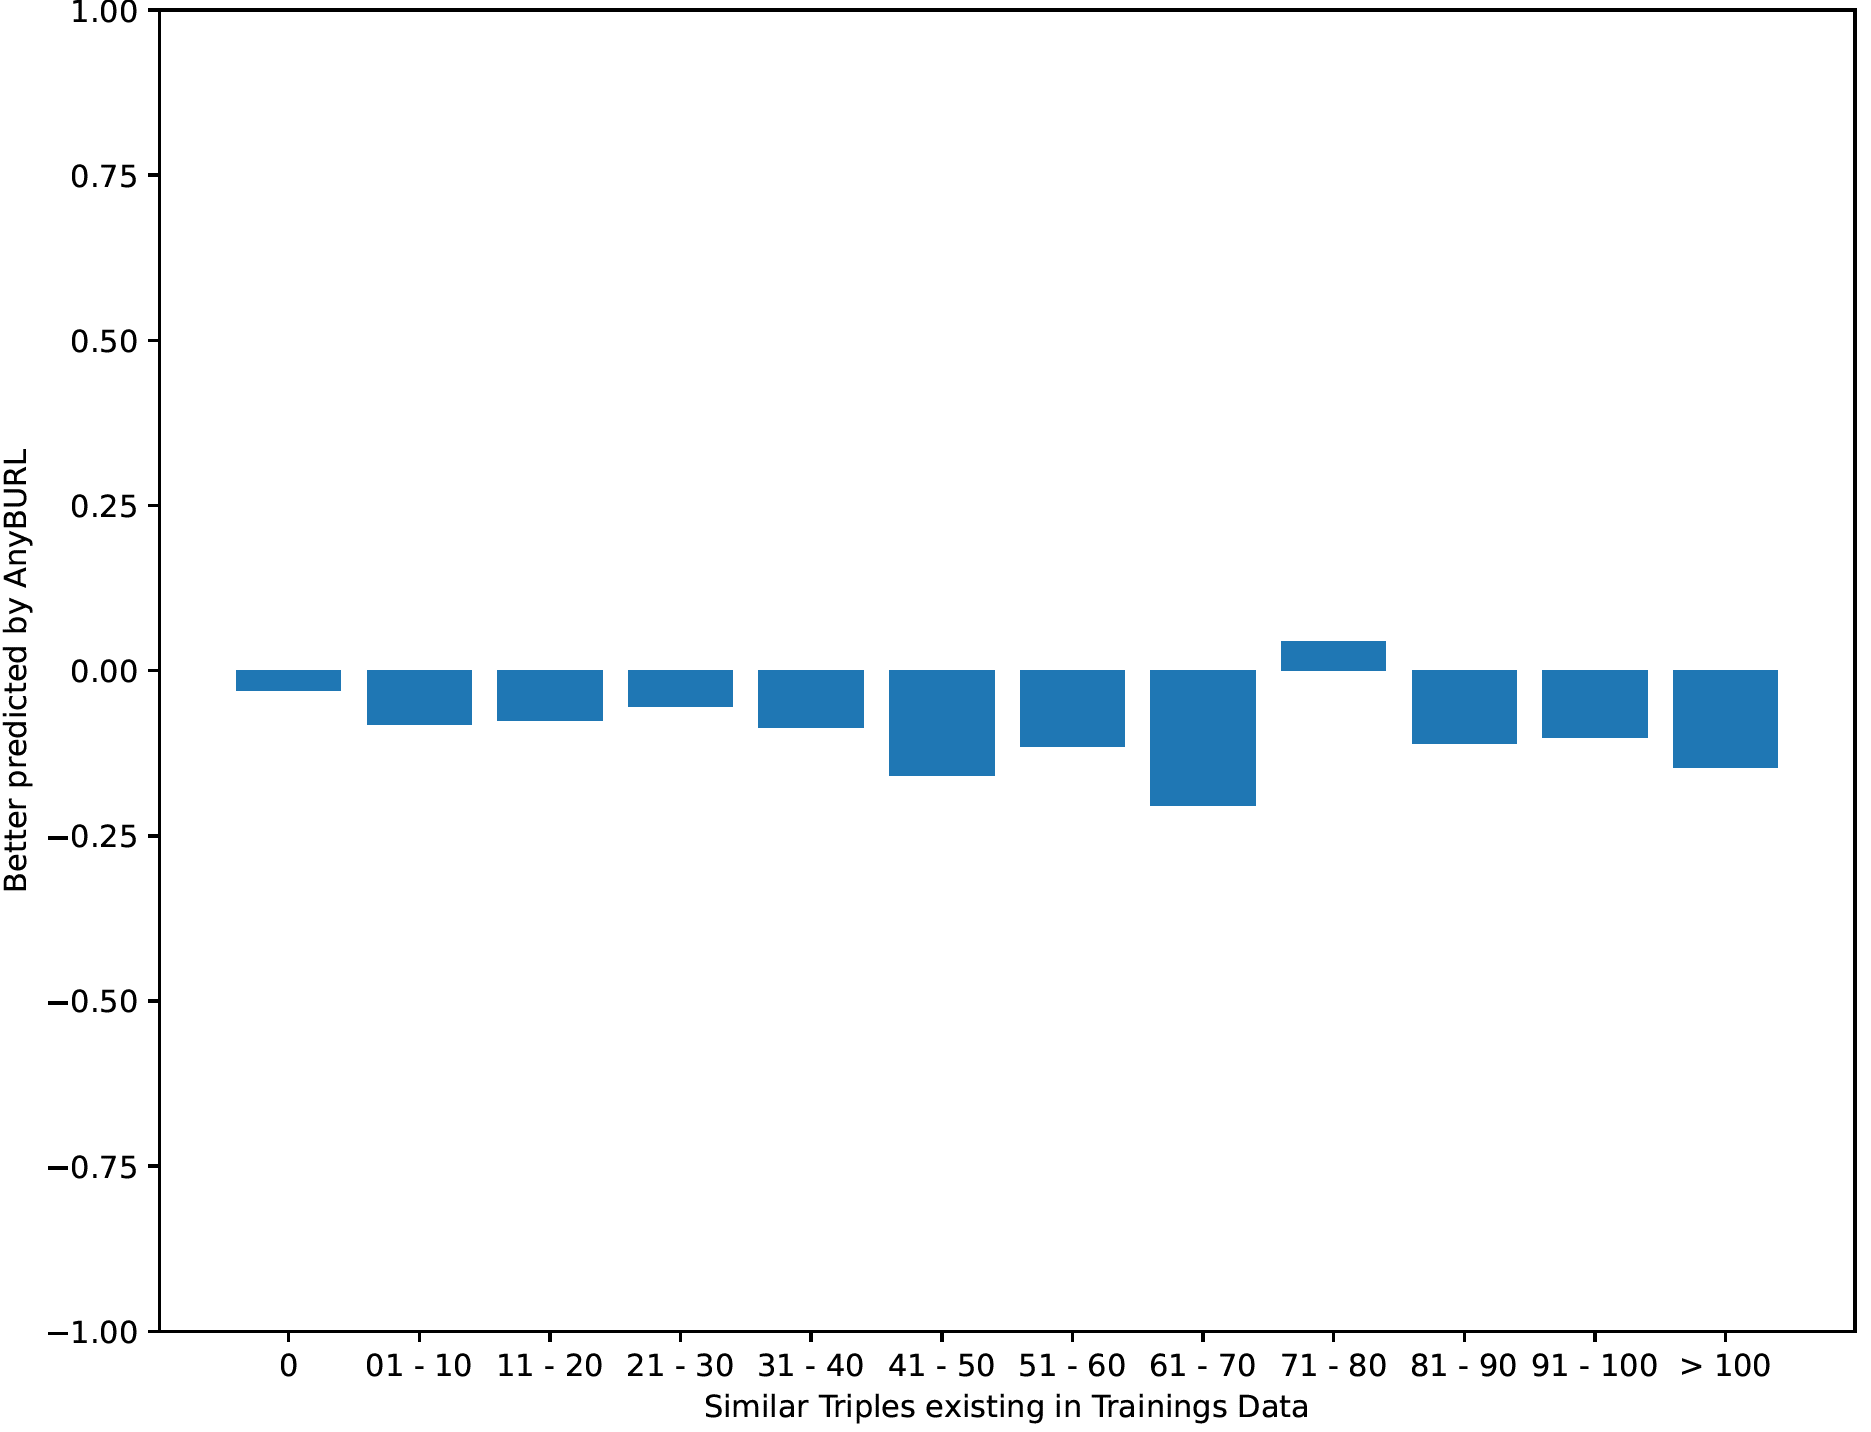
\includegraphics[width=0.7\textwidth]{images/similar_triples_steps_anyburl_conve_codex.PNG}
\caption{Comparison of AnyBURL and ConvE on FB15k-237 in regard to the amount of similar triples in the trainings data}
\label{fig:similar_triples_steps_anyburl_conve_fb15k}
\end{figure}

\begin{figure}[H]
\centering
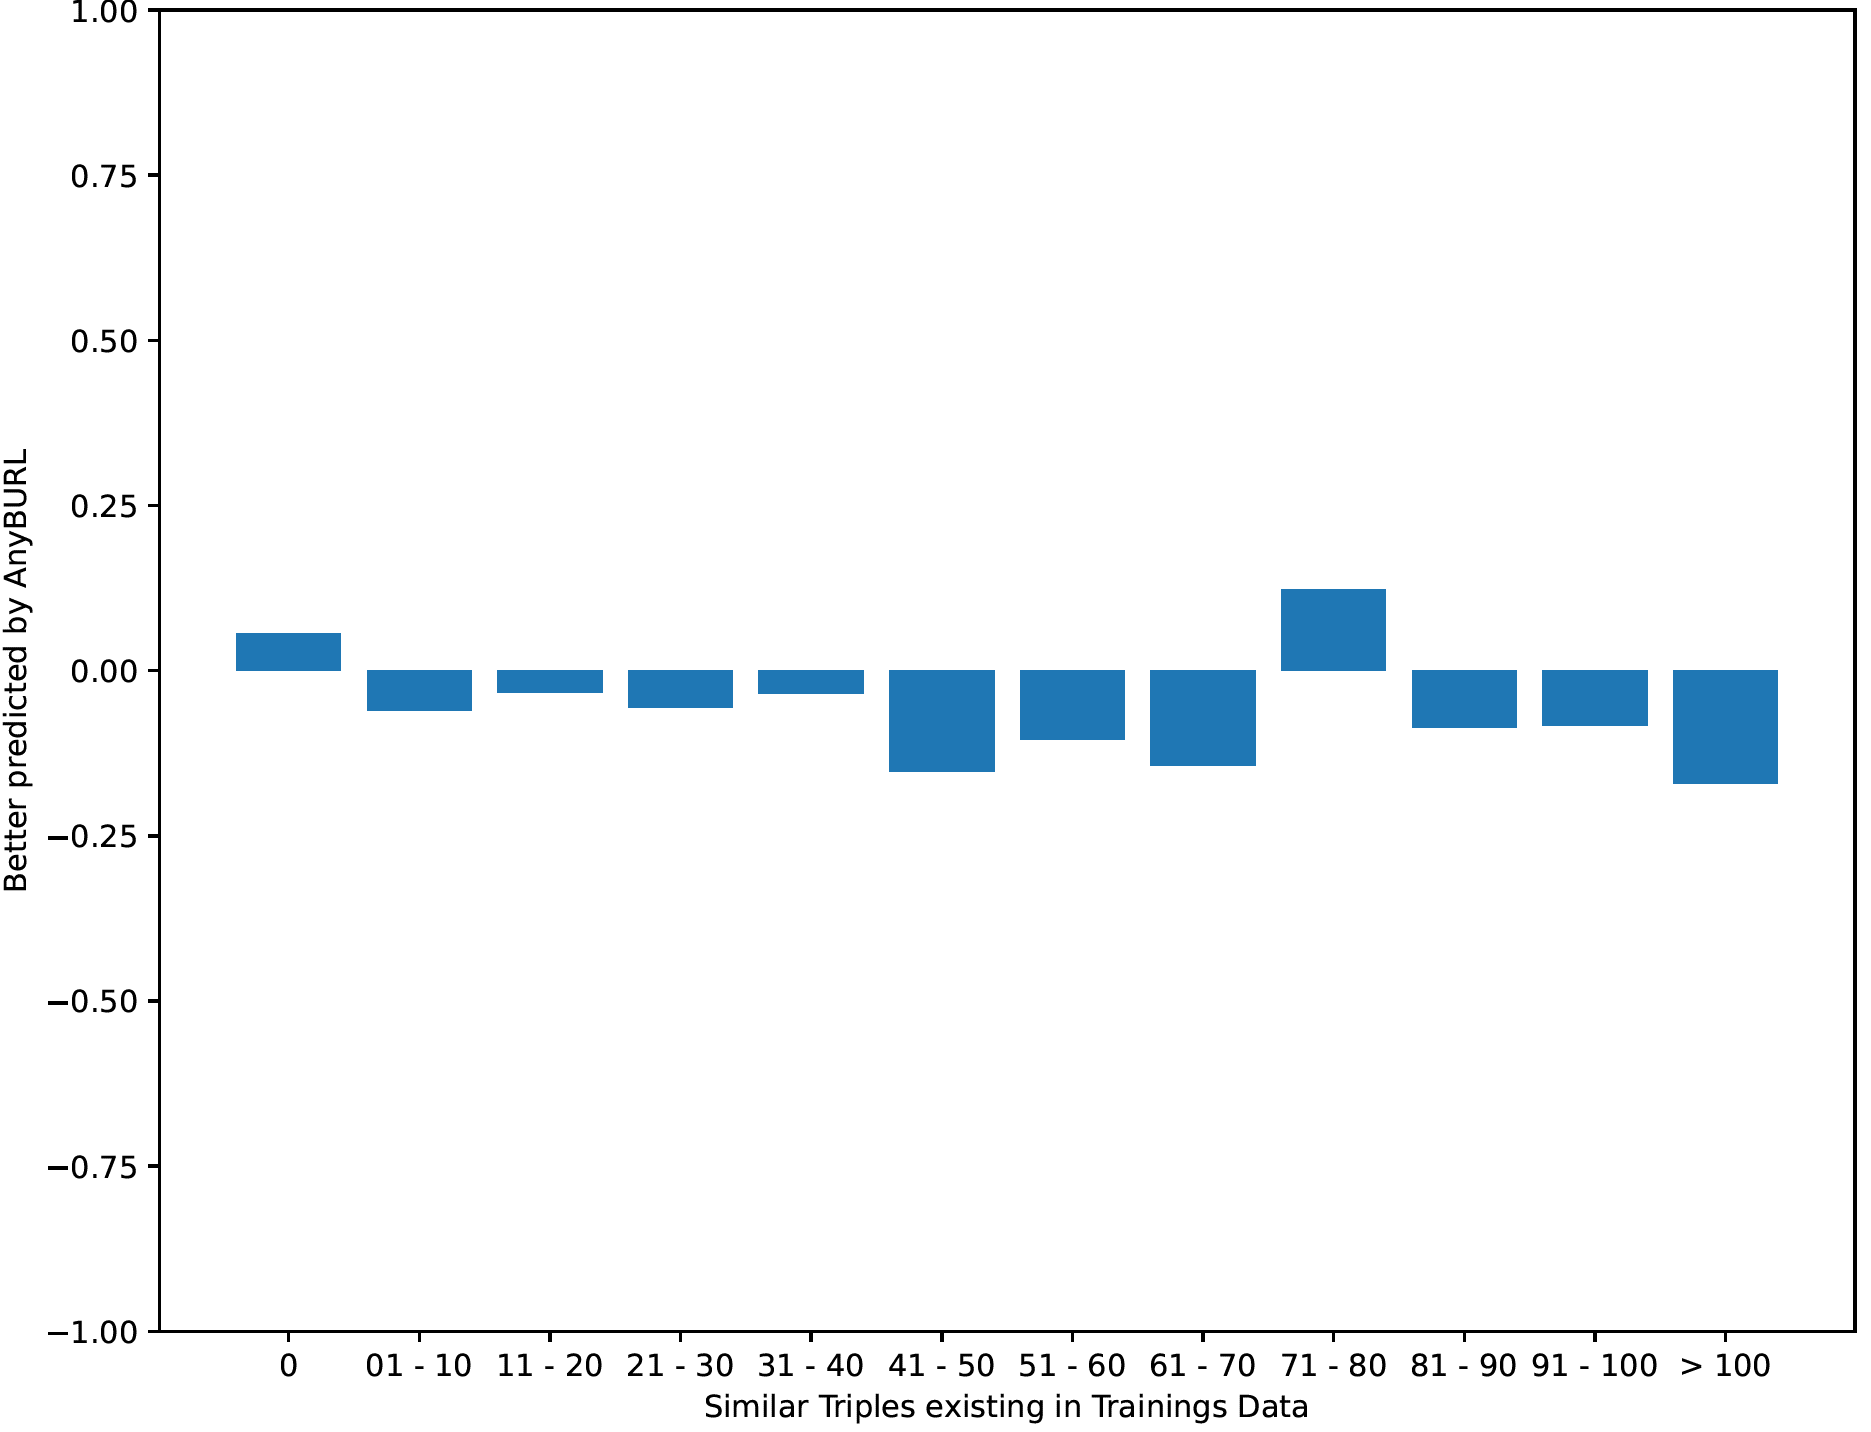
\includegraphics[width=0.7\textwidth]{images/similar_triples_steps_anyburl_rescal_codex.PNG}
\caption{Comparison of AnyBURL and RESCAL on FB15k-237 in regard to the amount of similar triples in the trainings data}
\label{fig:similar_triples_steps_anyburl_rescal_fb15k}
\end{figure}

\begin{figure}[H]
\centering
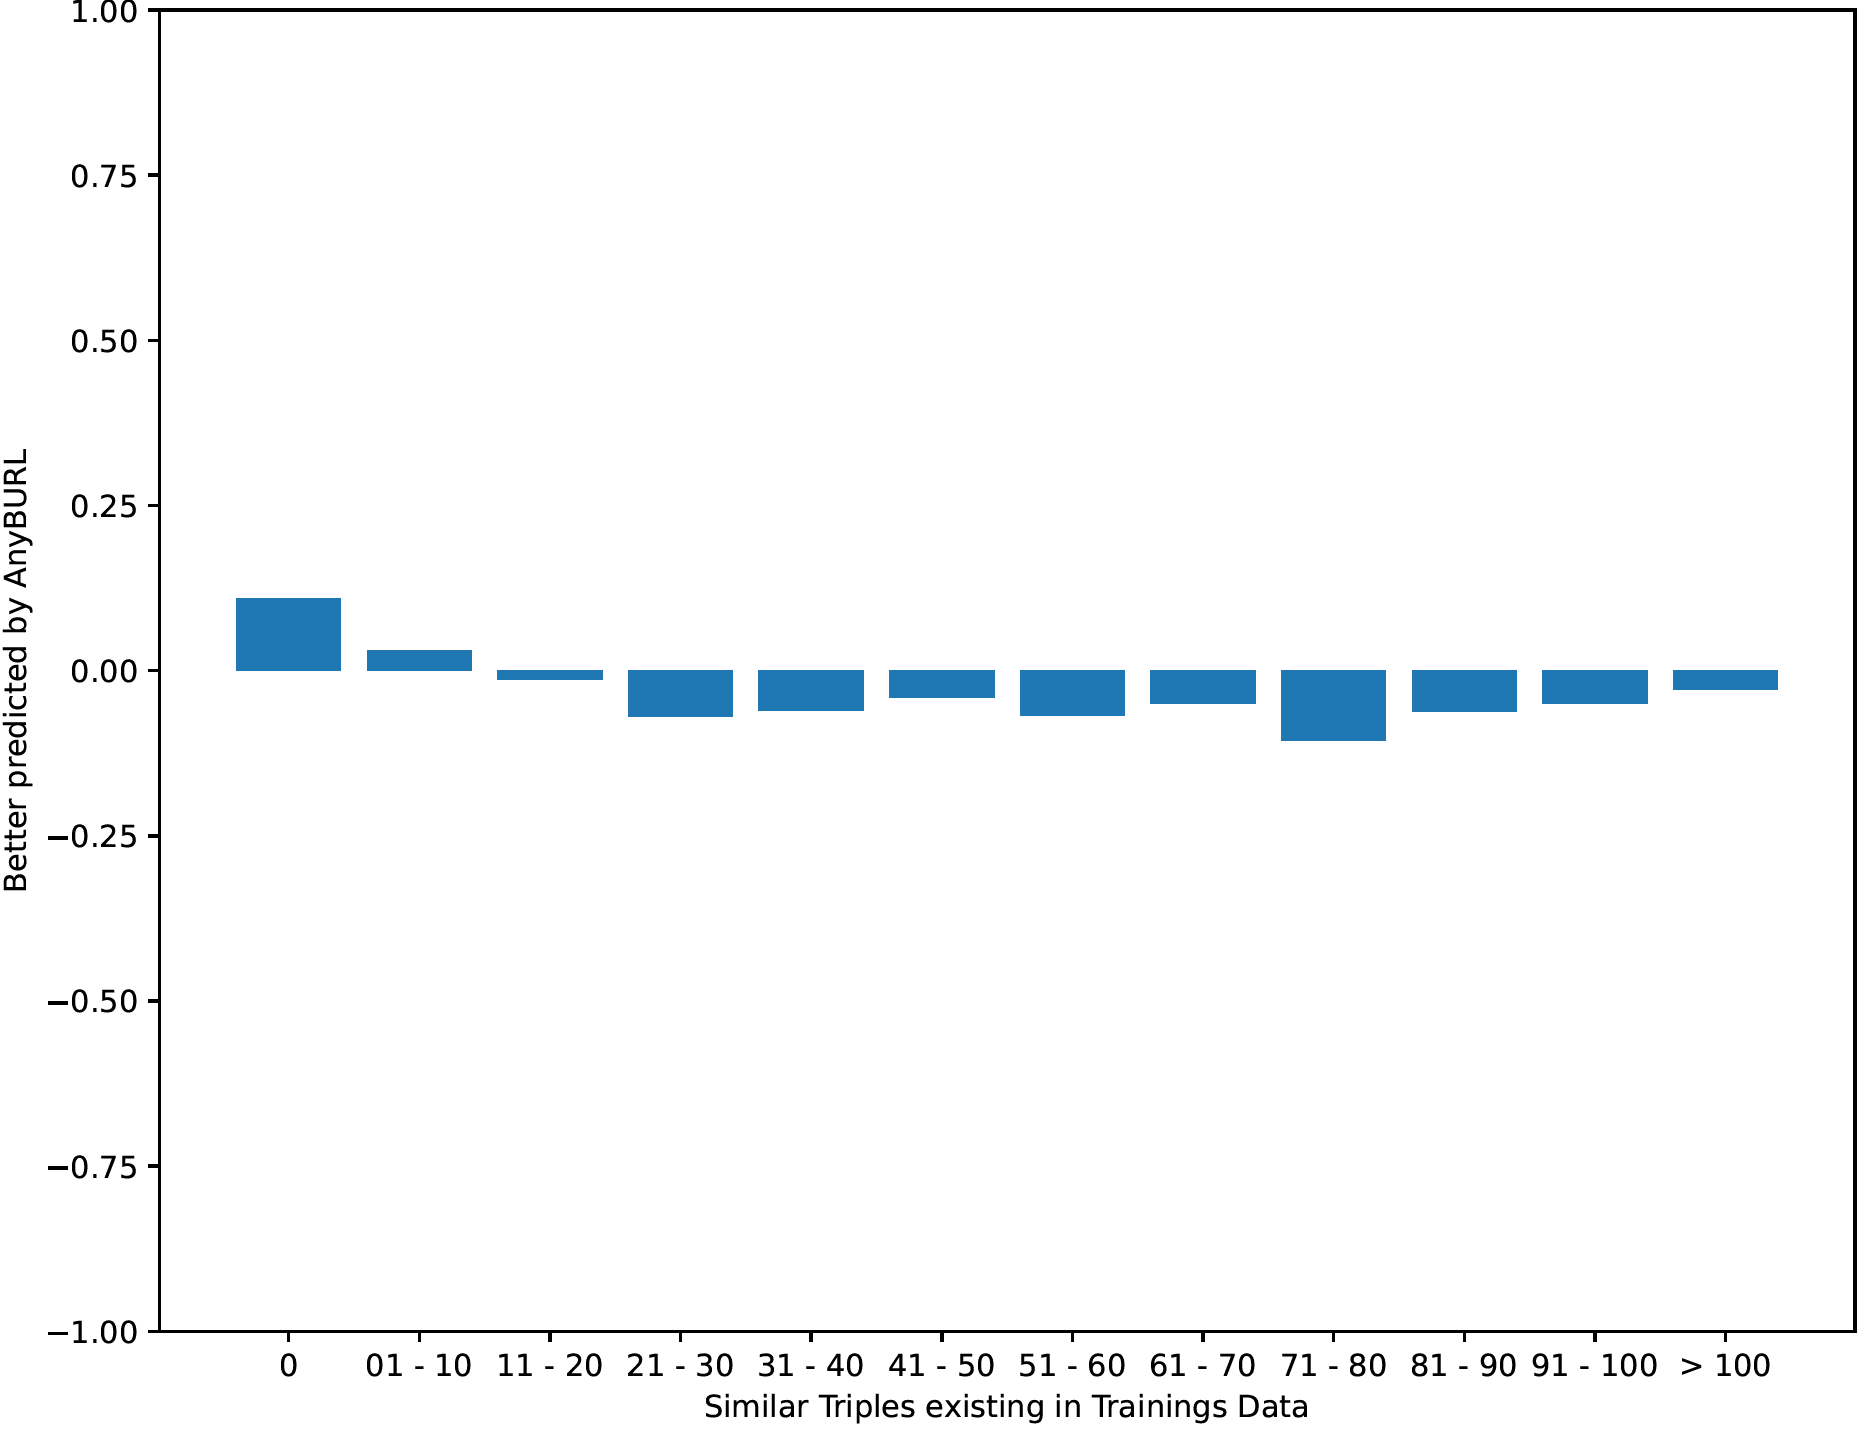
\includegraphics[width=0.7\textwidth]{images/similar_triples_steps_anyburl_complex_yago.PNG}
\caption{Comparison of AnyBURL and ComplEx on YAGO3-10 in regard to the amount of similar triples in the trainings data}
\label{fig:similar_triples_steps_anyburl_complex_yago}
\end{figure}

